% arara: xelatex: {synctex: true}
% arara: indent: {overwrite: yes}
\documentclass[]{IMTexam}

\usepackage[enums]{IMTtikz}

\givecredits
%\title{au}
\author{Isabella B.}
\USPN{11810773}
\date{}
\lecture{Física I} % disciplina
\lcode{4302111}
\hwtype{Resolução} % o que é
\examname{Lista 5} % prova

\begin{document}

\maketitle

\begin{questions}

	\question \label{ques:q1} Uma espingarda consiste em um cano horizontal, uma mola (de constante de mola $ k $ (\si{\newton\per\meter})) com extremidade fixa no extremo fechado do cano e um êmbolo que consiste de uma massa $ m $ presa à mola com coordenada $ x(t) $. Uma bala de massa $ M $(\si{\kilogram}) está inicialmente encostada na massa do êmbolo. Em $ t = 0 $ a mola que está comprimida até $ x(0) = −L $, é solta com velocidade inicial $ v_0 = 0 $ (\si{\meter\per\second}). Encontre a velocidade em que o êmbolo e a bala perdem contato. Despreze toda forma de atrito e viscosidade.

	\begin{solution}
		Pela lei de Hooke, a força elástica será dada por $ F_{el}=-k\,x $, e pela segunda lei de Newton, temos $ F_{el}=(m+M)\ddot{x} $. Portanto, temos uma equação diferencial de segunda ordem:
		\begin{equation}\label{eq:ddotSpring1}
			\ddot{x}+\dfrac{k}{m+M}\,x=0
		\end{equation}
		de solução geral $ x(t)=a\cos\omega\,t+b\sin\omega\,t $.

		Substituindo $ x $ pela solução geral em \ref{eq:ddotSpring1}:
		\[ -a\,\omega^{2}\cos\omega\,t-b\,\omega^{2}\sin\omega\,t+\dfrac{k}{m+M}\del{a\cos\omega\,t+b\sin\omega\,t}=0\implies \omega^{2}=\dfrac{k}{m+M} \]
		portanto,
		\begin{equation}\label{eq:omegaSpring}
			\omega=\sqrt{\dfrac{k}{(m+M)}}
		\end{equation}
		que é a frequência de oscilação da mola (para um período $ T $, $ \omega=2\pi/T $).

		Sendo $ x(0)=-L $, temos
		\[ -L=a\cos0+b\sin0\implies a=-L. \]

		Sendo $ \dot{x}(t)=v(t) $, e $ v(0)=v_0 $, temos%
		\footnote{Considerei $ v(0)=v_0 $ (por falta de atenção), e encontrei uma solução mais geral do que a pedida. Caso tenha dificuldade com alguma passagem, considere $ v_0=0 $, pois a situação se simplifica, e o problema será resolvido corretamente, independentemente.}%
		\[ v(t)=L\,\omega\sin\omega\,t+b\,\omega\cos\omega\,t\implies v(0)=v_0=L\,\omega\sin0+b\,\omega\,\cos0=b\,\omega\implies b=\dfrac{v_0}{\omega}. \]

		O que nos dá
		\begin{align}
			x(t)                          & =-L\cos\omega\,t+\dfrac{v_0}{\omega}\sin\omega\,t\label{eq:xSpring}                       \\
			v(t)             =\dot{x}(t)  & =L\,\omega\sin\omega\,t+v_0\cos\omega\,t\label{eq:vSpring1}                               \\
			a(t) =\dot{v}(t) =\ddot{x}(t) & =L\,\omega^{2}\cos\omega\,t-v_0\,\omega\sin\omega\,t=-\omega^{2}\,x(t)\label{eq:aSpring1}
		\end{align}

		Como queremos encontrar o momento de desprendimento, queremos encontrar o tempo $ t_d $ em que o conjunto êmbolo-bala tem velocidade máxima, já que, na ausência de atrito, após esse momento a bala terá $ v_{\text{máx}}>v_{\text{êmbolo}}(t) $ --- pois o êmbolo perde velocidade devido à força elástica --- e o conjunto se desprende.

		Para encontrar essa velocidade máxima, basta derivar $ v(t) $ e igualar a zero:
		\begin{align*}
			\dot{v}(t_d)                                                 & =0                                                                                                    \\
			\intertext{por \ref{eq:aSpring1}}
			a(t)=L\,\omega^{2}\cos\omega\,t_d-v_0\,\omega\sin\omega\,t_d & =0                                                                                                    \\
			\intertext{assumindo $ \cos\omega\,t_d\neq0 $}
			\dfrac{L\,\omega}{v_0}                                       & =\dfrac{\sin\omega\,t_d}{\cos\omega\,t_d}                                                             \\
			\tan\omega\,t_d                                              & =\dfrac{L\,\omega}{v_0}                                                                               \\
			t_d                                                          & =\dfrac{1}{\omega}\del{n\,\pi+\arctan\del{\dfrac{L\,\omega}{v_0}}}\quad\text{onde $ n\in\mathbb{N} $} \\
			\intertext{sendo $ n=0 $ (pois queremos a primeira solução), temos}
			t_d                                                          & =\dfrac{1}{\omega}\arctan\del{\dfrac{L\,\omega}{v_0}}
		\end{align*}

		Pela relação fundamental da trigonometria, temos
		\begin{align}
			\sin^{2}\theta+\cos^{2}\theta              & =1\nonumber                                                          \\
			\intertext{assumindo $ \sin\theta\neq0 $}
			1+\del{\dfrac{\cos\theta}{\sin\theta}}^{2} & =\dfrac{1}{\sin^{2}\theta}\nonumber                                  \\
			\dfrac{1}{\sin^{2}\theta}                  & =1+\dfrac{1}{\tan^{2}\theta}                                         \\
			\dfrac{1}{\sin^{2}\theta}                  & =\dfrac{\tan^{2}\theta+1}{\tan^{2}\theta}\nonumber                   \\
			\intertext{como $ \sin\theta\neq0\implies\tan\theta\neq0 $, podemos tomar o inverso dos dois lados}
			\sin^{2}\theta                             & =\dfrac{\del{\tan\theta}^{2}}{\del{\tan\theta}^{2}+1}\nonumber       \\
			\intertext{sendo $ \theta=\arctan x $}
			\sin^{2}\arctan x                          & =\dfrac{\del{\tan\arctan x}^{2}}{\del{\tan\arctan x}^{2}+1}\nonumber \\
			\intertext{pela propriedade da inversa, temos}
			\sin^{2}\arctan x                          & =\dfrac{x^{2}}{\del{x^{2}+1}}\nonumber                               \\
			\sin\arctan x                              & =\dfrac{|x|}{\sqrt{x^{2}+1}}\label{eq:senArctan}
		\end{align}

		Analogamente, para $ \cos\theta\neq0 $ e $ \theta=\arctan x $
		\begin{align}
			\cos^{2}\theta & =\dfrac{1}{\del{\tan\theta}^{2}+1}\nonumber    \\
			\cos\arctan x  & =\dfrac{1}{\sqrt{x^{2}+1}}\label{eq:cosArctan}
		\end{align}

		Substituindo $ t_d $ em \ref{eq:vSpring1}, temos
		\begin{align*}
			v(t_d) & =L\,\omega\sin\del{\omega\cdot\dfrac{1}{\omega}\arctan\del{\dfrac{L\,\omega}{v_0}}}+v_0\cos\del{\omega\cdot\dfrac{1}{\omega}\arctan\del{\dfrac{L\,\omega}{v_0}}}                         \\
			\intertext{por \ref{eq:senArctan} e \ref{eq:cosArctan}, temos}
			       & =L\,\omega\del{\dfrac{\envert{L\,\omega/v_0}}{\sqrt{\del{L\,\omega/v_0}^{2}+1}}}+v_0\del{\dfrac{1}{\sqrt{\del{L\,\omega/v_0}^{2}+1}}}                                                    \\
			\intertext{sendo $ L\,\omega/v_0>0 $}
			       & =L\,\omega\del{\dfrac{1}{\cancel{v_0^{-1}}}\dfrac{L\,\omega/\cancel{v_0}}{\sqrt{\del{L\,\omega}^{2}+v_0^{2}}}}+v_0\del{\dfrac{1}{v_0^{-1}}\dfrac{1}{\sqrt{\del{L\,\omega}^{2}+v_0^{2}}}} \\
			       & =\dfrac{\del{L\,\omega}^{2}+v_0^{2}}{\sqrt{\del{L\,\omega}^{2}+v_0^{2}}}=\sqrt{\del{L\,\omega}^{2}+v_0^{2}}                                                                              \\
			\intertext{substituindo \ref{eq:omegaSpring}, temos}
			       & =\sqrt{\del{L\,\sqrt{\dfrac{k}{\del{m+M}}}}^{2}+v_0^{2}}                                                                                                                                 \\
			v(t_d) & =\sqrt{\dfrac{k\,L^{2}+\del{m+M}v_0^{2}}{m+M}}
		\end{align*}

		\paragraph{Nota:} a resolução pedida pelo problema considera $ v_0=0 $, portanto, $ v(t_d) =\sqrt{k/\del{m+M}}L $.
	\end{solution}

	%	

	\question A Figura \ref{fig:fig1} mostra um conjunto de massas sólidas. Há uma força $\vec{F}$ na direção indicada. Não há atrito entre nenhuma superfície. A polia e a corda são ideais (sem massa e de comprimento constante). Encontre a força $\vec{F_0}$ como função das massas $ M_1, M_2 $ e $ M_3 $ para que a massa 3 não suba nem desça num campo gravitacional onde a aceleração é $g$ para baixo. O que acontece (calcule o movimento vertical de $ M_3 $) se a força for $ \vec{F_0} + \Delta \vec{f} $? Discuta a relação entre o sinal, (sentido) de $ \Delta\vec{f} $ e a movimento de $ M_3 $.

	\begin{figure}[H]
		\centering
		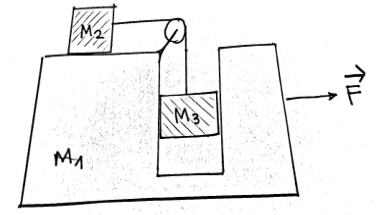
\includegraphics[width=0.4\linewidth]{screenshot001}
		\caption{Conjunto de massas sólidas.}
		\label{fig:fig1}
	\end{figure}

	\clearpage

	\by{Anahí}

	\begin{solution}
		Escrevendo a resultante das forças para cada massa, temos:
		\begin{align}
			\vec{F_1} & =\vec{F_0}+\vec{N_{3\,1}}+\vec{T}\label{eq:block1Fr} \\
			\vec{F_2} & =\vec{T}\label{eq:block2Fr}                          \\
			\vec{F_3} & =\vec{F_0}+\vec{P_3}+\vec{T}\label{eq:block3Fr}
		\end{align}
		onde $\vec{N_{3\,1}}$ é a força normal aplicada pelo bloco 3 sobre o bloco 1, $ \vec{P_3} $ é o peso do bloco 3 e $ \vec{T} $ é a tensão da corda.

		Adotemos a notação do módulo de um vetor $ \vec{v} $ por $ |\vec{v}|=v $.

		Pelo enunciado, temos que a aceleração do bloco 3 na vertical deve ser zero e, tomando \ref{eq:block3Fr}, pela segunda Lei de Newton, temos:
		\begin{equation}\label{eq:f3yQ2}
			F_{3y}=M_3\,a_{3y}\implies P_3-T=0\implies T=M_3\,g
		\end{equation}

		Como $ a_{3y}=0 $, por \ref{eq:block3Fr}:
		\[ F_3=N_{3\,1}  \]
		A partir disso, podemos achar a relação entre a aceleração $ \vec{a} $ do conjunto, por \ref{eq:block1Fr} e \ref{eq:block2Fr}:
		\begin{align*}
			F_1                & =F_0-N_{3\,1}-T=F-F_3-F_2           \\
			F_0                & =F_1+F_2+F_3                        \\
			\intertext{aplicando a segunda lei de Newton}
			\del{M_1+M_2+M_3}a & =M_1\,a_1+M_2\,a_2+M_3\,a_3\implies \\
			a                  & =a_1=a_2=a_3
		\end{align*}

		Como todas as acelerações são iguais, substituindo \ref{eq:f3yQ2} em \ref{eq:block2Fr} e, pela segunda lei de Newton, temos:
		\begin{equation}\label{eq:accVQ2}
			F_{2}=T\implies M_2\,a=M_3\,g\implies a=\dfrac{M_3}{M_2}g
		\end{equation}

		Portanto, como $ F_0=M_t\,a $ ($ M_t $ sendo a massa total), temos:
		\[ \boxed{F_0=\del{M_1+M_2+M_3}\dfrac{M_3}{M_2}g.} \]

		Para $ \vec{F}=\vec{F_0}+\Delta\vec{f} $, como, por \ref{eq:block1Fr}, a nova tensão $ |\vec{T'}|=\envert{\vec{F_1}-\vec{N_{3\,1}}-\vec{F}}=\envert{\vec{F_1}-\vec{N_{3\,1}}-\del{\vec{F_0}+\Delta\vec{f}}}<|\vec{T}| $ --- supondo $ \Delta\vec{f} $ no sentido de $ x $ positivo --- a aceleração do bloco 2 tende a diminuir, o que levaria o bloco 3 a se deslocar para cima.
	\end{solution}



	\question Encontre a frequência de oscilação de uma massa presa a duas molas
	ligadas:

	\begin{parts}
		\part em paralelo;

		\part em série.

	\end{parts}

	Dados: $ M, k_1, k_2 $.

	\clearpage

	\begin{solution}
		Temos que a força elástica de cada mola será $ F_{el\,1}=-k_1\,x_1 $ e $ F_{el\,2}=-k_2\,x_2 $, pela lei de Hooke.

		Partindo disso:
		\begin{enumerate}[label=(\alph*)]
			\item Para o caso da ligação em paralelo:

			      Como as molas estão em paralelo, sua deformação será idêntica (vamos denotá-la por $ X_p $). Sendo a força elástica sobre a mola equivalente às duas em paralelo $ F_{el\,p}=-k_{eq\,p}\,X_p=F_{el\,1}+F_{el\,2} $, temos
			      \[ F_{el\,p}=F_{el\,1}+F_{el\,2}\implies -k_{eq\,p}\,X_p=-k_1\,X_p-k_2\,X_p\implies k_{eq\,p}=k_1+k_2. \]

			      Pela equação \ref{eq:omegaSpring}, temos:
			      \begin{equation}\label{eq:freqPara}
				      \omega_{p}=\sqrt{\dfrac{k_1+k_2}{M}}
			      \end{equation}

			\item Para o caso da ligação em série:

			      Se considerarmos a massa das molas desprezível, a força elástica sobre a mola equivalente às duas em série é dada por $ F_{el\,s}=-k_{eq\,s}\,X_s=F_{el\,1}=F_{el\,2} $%
			      \footnote{Podemos imaginar duas molas em série apoiando um livro sobre uma mesa, a mola de cima é pressionada pelo peso do livro, e a mola de baixo é pressionada pelo peso do livro e pelo peso da outra mola, que deve ser desprezível, logo, ambas sofrem a mesma força (de \url{https://physics.stackexchange.com/questions/311111/why-springs-in-series-experience-equal-force}).}.

			      Como a deformação total $ X_s=x_1+x_2 $, temos
			      \[ -\dfrac{F_{el\,s}}{k_{eq\,s}}=-\dfrac{F_{el\,1}}{k_1}-\dfrac{F_{el\,2}}{k_2}\implies k_{eq\,s}=\dfrac{k_1\,k_2}{k_1+k_2} \]

			      Por \ref{eq:omegaSpring}, temos:
			      \begin{equation}\label{eq:freqPerp}
				      \omega_{p}=\sqrt{\dfrac{k_1\,k_2}{M\del{k_1+k_2}}}
			      \end{equation}
		\end{enumerate}
	\end{solution}

	\question Um carro tem aceleração constante $\vec{A}$. Em $ t = 0 $ jogo uma bola para frente num ângulo $\theta$ e a bola cai, em $ t = T^{\star} $ exatamente no lugar de onde foi lançada no carro. Para que valores de $ \theta, \vec{v_0} $ e $\vec{V_C}$ isso é possível? $\vec{v_0}$ e $\vec{V_C}$ são, respectivamente, a velocidade medida em relação ao carro no momento em que a bola é jogada e a velocidade do carro em
	$ t = 0 $. Como sempre a aceleração da gravidade tem intensidade $ g = |\vec{g}| $.

	\begin{solution}

		\begin{multi}
			Sendo $\vec{v_c}$ a velocidade da bola no referencial do carro, por transformações de Galileu, sabemos que a velocidade da bola $ \vec{v_b} $ no referencial externo é
			\[ \vec{v_b}=\vec{v_c}+\vec{v} \]
			e, sendo a velocidade do carro no tempo $ \vec{v} $ e a aceleração da bola em relação ao carro $ \vec{a_c} $, temos que a aceleração da bola em relação ao referencial externo $ \vec{a_b} $ será
			\[ \vec{a_b}=\dod{}{t}\sbr{\vec{v_c}+\vec{v}}=\vec{a_c}+\vec{A} \]

			%			Sendo o vetor velocidade do carro no tempo
			%			\[ \vec{v}(t)=\vec{V_C}+\int_{0}^{t}\vec{A}\,\dif\tau=\vec{V_C}+\vec{A}\,t \]

			\nextcol
			\centering
			\begin{tikzpicture}
				\coordinate (Si) at (0,0);
				\draw[->] (Si)++(-0.5,0) -- +(2,0);
				\draw[->] (Si)++(0,-0.5) -- +(0,2);
				\node[below left] at (Si) {Exterior};

				\coordinate (Sd) at (3,2);
				\draw[->] (Sd)++(-0.5,0) -- +(2,0);
				\draw[->] (Sd)++(0,-0.5) -- +(0,2);
				\node[below right] at (Sd) {Carro};

				\coordinate (obj) at (1,3);
				\draw[-Latex] (Si) -- node[above left] {$ \vec{v_b} $} (obj);
				\draw[-Latex] (Sd) -- node[above right] {$ \vec{v_c} $}(obj);
				\draw[-Latex] (Si) -- node[below right] {$ \vec{v} $} (Sd);

				\filldraw (obj) circle (2pt) node[above] {Bola};
			\end{tikzpicture}
		\end{multi}



		Para $ t<0 $ sabemos que a bola está parada dentro do carro --- onde temos uma força resultante das interações dentro do carro $ \vec{F_{r\,0}} $, e uma força fictícia $ \vec{F_F} $ --- portanto, pela segunda lei de Newton:
		\[ \vec{F_{r\,0}}+\vec{F_F}=\vec{0}\implies \vec{F_F}=-m\,\vec{A}. \]

		Quando jogamos a bola (portanto, $ t>0 $), no referencial do carro, há uma força $ \vec{F_r} $ aplicada na bola que é a soma do peso da bola $ \vec{P} $ e da força fictícia $ \vec{F_F} $, e, pela segunda lei de Newton, temos:
		\[ \vec{F_r}=\vec{F_F}+\vec{P}\implies m\,\vec{a_c}=m\del{-\vec{A}+\vec{g}}, \]
		pois a aceleração resultante no referencial do carro é $\vec{a_c}$. Isso implica que \[ \vec{a_c}=\vec{g}-\vec{A}. \]

		%		Quando jogamos a bola para frente com velocidade $ \vec{v_c}=\vec{v_b}-\vec{v} $, a bola sofrerá uma aceleração $ \vec{a_c}=\vec{a_b}-\vec{A} $ enquanto estiver no ar.

		O vetor velocidade $ \vec{v_c}(t) $ será a integral da aceleração $\vec{a_c}(t)$ no tempo:
		\[ \vec{v_c}(t)=\int \vec{a_c}(t)\dif t=\int \vec{g}-\vec{A}\dif t=\del{\vec{g}-\vec{A}}t+C_1 \]
		como $ \vec{v_c}(0)=\vec{v_0} $, pelo enunciado, temos $ C_1=\vec{v_0} $.

		O vetor posição da bola no tempo no referencial do carro $ \vec{r_c}(t) $ será a integral de $ \vec{v_c}(t) $ no tempo:
		\begin{align*}
			\vec{r_c}(t) & =\int \vec{v_c}\dif t                                    \\
			             & =\int \del{\vec{g}-\vec{A}}t+\vec{v_0} \dif t            \\
			\vec{r_c}(t) & =\dfrac{1}{2}\del{\vec{g}-\vec{A}}t^{2}+\vec{v_0}\,t+C_2
		\end{align*}
		Chamemos $\vec{r_c}(t=0)=\vec{r_0}$, isso implica em $ C_2=\vec{r_0} $.

		Como $ \vec{r_c}(t=T^{\star})=\vec{r_0} $ --- pelo enunciado ---, temos:
		\[ \vec{r_c}(T^{\star})=\dfrac{1}{2}\del{\vec{g}-\vec{A}}T^{\star\,2}+\vec{v_0}\,T^{\star}+\vec{r_0}=\vec{r_0}\implies \del{\dfrac{1}{2}\del{\vec{g}-\vec{A}}T^{\star}+\vec{v_0}}T^{\star}=0, \]
		portanto, $ T^{\star}=0 $ ou
		\begin{equation}\label{eq:TstarVec}
			\dfrac{1}{2}\del{\vec{g}-\vec{A}}T^{\star}+\vec{v_0}=0\implies \del{\vec{A}-\vec{g}}T^{\star}=2\vec{v_0}
		\end{equation}

		Adotemos a notação $ |\vec{v}|=v $, e um eixo de coordenadas $ x-y $ com $ x $ na horizontal, na mesma direção e sentido da aceleração do carro, e $ y $ na vertical e com sentido oposto ao da gravidade.

		Assumindo que a bola foi lançada com um ângulo $ \theta $ em relação à horizontal, $ |\vec{v_{0x}}|=v_0\cos\theta $ e $ |\vec{v_{0y}}|=v_0\sin\theta $ são os módulos das componentes de $\vec{v_0}$ na horizontal e na vertical, respectivamente, temos, por \ref{eq:TstarVec}:
		\begin{gather}
			A\,T^{\star}=2v_0\cos\theta\implies T^{\star}=\dfrac{2v_0\cos\theta}{A}\label{eq:Tstar1}\\
			g\,T^{\star}=2v_0\sin\theta\implies
			T^{\star}=\dfrac{2v_0\sin\theta}{g}\label{eq:Tstar2}
		\end{gather}
		Igualando%
		\footnote{Alternativamente, podemos somar os quadrados de \ref{eq:Tstar1} e \ref{eq:Tstar2}: $ \del{g^{2}+A^{2}}T^{\star2}=4v_0^{2}\del{\sin^{2}\theta+\cos^{2}\theta}\implies T^{\star}=2v_0/\del{\sqrt{g^{2}+A^{2}}} $.}%
		\ref{eq:Tstar1} e \ref{eq:Tstar2}, temos
		\begin{align*}
			\dfrac{2v_0\sin\theta}{g} & =\dfrac{2v_0\cos\theta}{A}   \\
			\intertext{para $ \cos\theta\neq0 $}
			\tan\theta                & =\dfrac{g}{A}                \\
			\theta                    & =\arctan \del{\dfrac{g}{A}}.
		\end{align*}
		Substituindo em \ref{eq:Tstar1}, temos
		\begin{align*}
			T^{\star} & =\dfrac{2v_0\cos\arctan \del{g/A}}{A}    \\
			\intertext{por \ref{eq:cosArctan}, temos}
			          & =\dfrac{2v_0}{A\,\sqrt{\del{g/A}^{2}+1}} \\
			T^{\star} & =\dfrac{2v_0}{\sqrt{g^{2}+A^{2}}}
		\end{align*}

		Como nossas contas não dependem de $\vec{V_C}$, ele pode ser um valor arbitrário. Já $ |\vec{v_0}|>0 $, pois $T^{\star}\stackrel{!}{>}0$.
	\end{solution}



	\question Uma lavadora de vidros externos de um prédio está sentada em uma cadeira de cabos. Suponha que a única forma de movimento é na vertical. A massa da mulher é $ M $ e a da cadeira $ m $. O cabo passa por uma polia e volta até ela, que pode puxar o cabo para subir. Ela puxa o cabo para baixo com tal força que a força que faz na cadeira é $ N $.

	\begin{figure}[H]
		\centering
		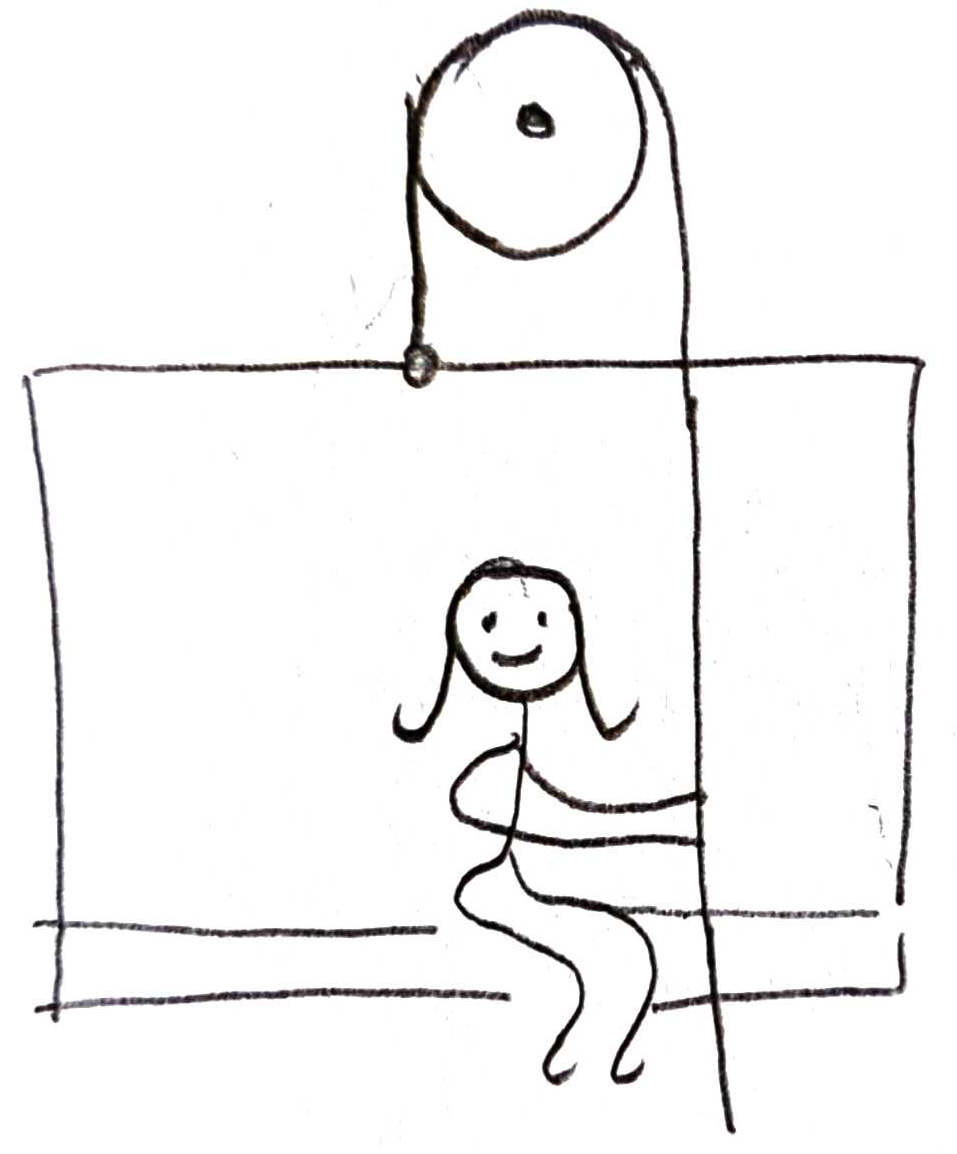
\includegraphics[width=0.4\linewidth]{screenshot002}
		\caption{Lavadora de vidros sentada na cadeira de cabos.}
		\label{fig:fig2}
	\end{figure}

	\begin{parts}
		\part Qual é a aceleração da lavadora e da cadeira?
		\part Qual é a força sobre a polia?
	\end{parts}

	Faça o diagrama de forças e no final do exercício substitua os valores
	$ N = 300\,\text{newtons}, M = \SI{60}{\kilogram}, m = \SI{10}{\kilogram} $ e $ g = \SI{10}{\meter\per\second\squared}$.

	\clearpage

	\begin{solution}

		\begin{multi}
			\begin{unindent}
				\item Sendo a massa total do sistema mulher-cadeira $ M+m $, sendo $ F_r $ a força resultante no sistema e $ P $ o peso do conjunto, pela segunda lei de Newton, em módulo, temos:
				\begin{align}
					F_r  & =(M+m)a\nonumber                               \\
					2N-P & =(M+m)\,a\nonumber                             \\
					a    & =\dfrac{2N-(M+m)g}{M+m} \label{eq:aWomanChair}
				\end{align}
				Pois a força de reação da corda sobre a mulher faz com que a força $ N $ atue duas vezes no sistema.
				\item A força sobre a polia $ F_p $ deve ser igual à soma da força aplicada pela mulher, e a força peso sofrida pelo conjunto:
				\begin{equation}\label{eq:FpWC}
					F_p=N+P=N+(M+m)g
				\end{equation}
			\end{unindent}

			\nextcol

			\centering
			\begin{tikzpicture}
				\node (M) at (0,0) {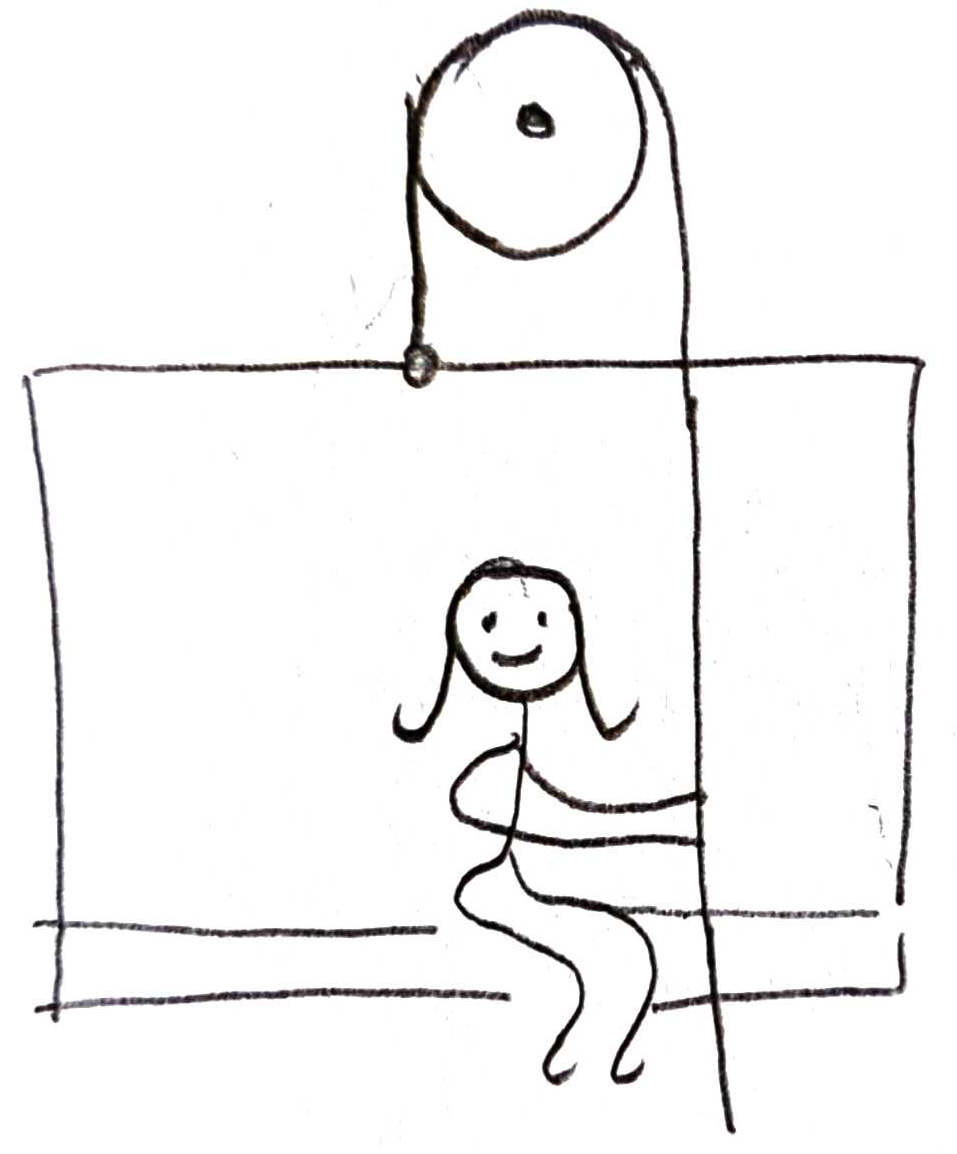
\includegraphics[scale=0.2]{screenshot002}};

				\coordinate (P) at (-0.5,2.5);
				\coordinate (N) at (1.25,2.5);
				\coordinate (NonC) at (-1,-2);
				\coordinate (PonC) at (-0.75,-2);
				\coordinate (TonG) at (1,-1.2);
				\coordinate (GonT) at (1.4,-1.5);

				\draw[thick,red,-Latex] (P) -- node[left] {$ P $} +(0,-1);
				\draw[thick,red,-Latex] (PonC) -- node[left] {$ P $} +(0,-1);
				\draw[thick,red,-Latex] (N) -- node[right] {$ N $} +(0,-1);
				\draw[thick,red,-Latex] (NonC) -- node[right] {$ N $} +(0,1);

				\draw[thick,red,-Latex] (TonG) -- +(0,1) node[above] {$ N $};
				\draw[thick,red,-Latex] (GonT) -- node[right] {$ N $} +(0,-1);
			\end{tikzpicture}
		\end{multi}



		Substituindo os valores dados em \ref{eq:FpWC} e \ref{eq:aWomanChair}, temos
		\begin{gather*}
			a=\dfrac{2\cdot300-(60+10)10}{60+10}=-\SI{1.42}{\meter\per\second\squared}\\
			F_p=300-(60+10)10=-\SI{400}{\newton}
		\end{gather*}
	\end{solution}



	\question Considere um pêndulo: uma massa $ m $ presa por um fio sem massa de
	comprimento $ l_0 $ a temperatura $ T_0 $ , num campo gravitacional uniforme.

	\begin{enumerate}[label=\arabic*.]
		\item Mostre as forças atuantes no sistema.
		\item Escreva as equações de movimento.
		\item Sob hipótese de amplitudes pequenas de movimento, o ângulo com a vertical satisfaz $ \tan(\theta) \approx \theta $. Nestas condições resolva as equações de movimento, isto é, encontre $\theta(t)$ para as condições iniciais $ \theta(t = 0) = \theta_0 $ e $ \od{\theta}{t}(t=0)=u $.
		\item  Suponha que $ l $ é afetado pela temperatura. O coeficiente linear de 	expansão é $ \alpha $, de forma que $ l(T) = l_0(1+\alpha(T −T_0)) $. Como muda 	o período do pêndulo com a temperatura? Faça a aproximação 	que $ |\alpha(T − T_0)| \ll 1 $.
		\item Olhe novamente para as equações de movimento e mantenha a temperatura fixa em $ T_0 $. Faça um argumento para indicar se o período aumenta ou diminui se a amplitude for maior e a aproximação de baixos ângulos deixar de valer.
	\end{enumerate}

	\clearpage

	\begin{solution}

		\topenum
		\begin{multi}
			\centering
			\begin{tikzpicture}[scale=1.5]
				%				\draw[->] (-2,-3) -- +(4,0) node[right] {$ x $};
				%				\draw[->] (0,-4) -- (0,-1.5) node[above] {$ y $};
				%				
				%				\draw[thick,-Latex] (0,-3) -- node[below] {$ \ihat $} +(1,0);
				%				\draw[thick,-Latex] (0,-3) -- node[left] {$ \jhat $} +(0,1);

				\fill[pattern={north west lines}] (-1,0) rectangle +(1.75,0.5);
				\draw[white,line width=3pt] (0,0) -- (0,-0.5) (0,0) -- +(30:1);
				\draw (-1,0) -- +(1.75,0);
				\draw[thick] (0,0) -- +(-60:3) coordinate (m);
				\draw[-Latex,red,thick] (m) -- +(0,-1) coordinate (P) node[right] {$ \vec{P} $};
				\draw[-Latex,red,thick] (m) -- +(120:1) node[right=3pt] {$ \vec{T} $};
				\fill (m) circle (2pt);
				\draw[dashed] (0,0) coordinate (O) -- +(0,-0.75) coordinate (A) (0,0) -- +(30:1) (m) -- +(30:1);
				\draw[|<->|] (120:0.2pt)++(30:1) -- node[fill=white,inner sep=1pt] {$ l $} +(-60:3cm+0.4pt);

				\pic[draw=black, angle radius=25pt,angle eccentricity=1,"$ \theta $" {xshift=2pt,yshift=-7pt}] {angle=A--O--m};

				\draw[dashed] (m) -- +(120:-0.5) coordinate (B);

				\pic[draw=black, angle radius=15pt,angle eccentricity=1,"$ \theta $" {xshift=1pt,yshift=-5pt}] {angle=P--m--B};
			\end{tikzpicture}

			\nextcol

			Aplicando a segunda lei de Newton para as forças no diagrama, temos:
			\begin{equation}\label{eq:PTma}
				\vec{P}+\vec{T}=m\,\vec{a}
			\end{equation}
			Sendo o movimento resultante similar à um movimento circular, podemos analisar as componente tangencial e radial de \ref{eq:PTma}.
			Sabemos que a velocidade tangencial será dada por $ v_t=l\,\od{\theta}{t} $, e sua aceleração tangencial $ a_t=l\,\od[2]{\theta}{t} $ supondo que $ l $ é constante no tempo.

			Pela componente tangencial, temos:
			\begin{equation}\label{eq:tangMot}
				-m\,g\sin\theta=m\,l\,\dod[2]{\theta}{t}
			\end{equation}
			onde $ \theta $ é o ângulo formado entre o fio de comprimento $ l $ e a vertical, como no diagrama ao lado.
		\end{multi}

		\begin{unindent}
			\item Se o ângulo satisfaz $ \tan\theta\approx\theta $, segue que $ \sin\theta\approx\theta $ também. Portanto, a partir de \ref{eq:tangMot}, temos:
			\[ m\,l\,\dod[2]{\theta}{t}\approx-m\,g\,\theta\implies \dod[2]{\theta}{t}+\dfrac{g}{l}=0 \]
			O que é uma equação com solução geral do oscilador harmônico simples, no formato de $ \theta(t)=a\cos\omega\,t+b\sin\omega\,t $, com $ \omega=\sqrt{g/l} $.
			Pelas condições iniciais, temos:
			\[ \theta(0)=a=\theta_0 \]
			e
			\[ \dot{\theta}=-a\,\omega\sin\omega\,t+b\,\omega\cos\omega\,t\implies \dot{\theta}=b\,\omega=u\implies b=\dfrac{u}{\omega} \]
			Portanto:
			\begin{equation}\label{eq:thetat}
				\theta(t)=\theta_0\cos\omega\,t+\dfrac{u}{\omega}\sin\omega\,t.
			\end{equation}

			\item Sendo $ l $ uma função da temperatura $ T $, tal que
			\begin{equation}\label{eq:deltaLdeltaT}
				l(T)=l_0\del{1+\alpha\del{T-T_0}}
			\end{equation}
			onde $ T_0 $ e $ l_0 $ são a temperatura inicial e o comprimento inicial do fio, respectivamente, como $ \omega=\sqrt{g/l} $, e o período $ p=2\pi/\omega $, temos
			\begin{equation}\label{eq:periodPend}
				p(T)=2\pi\sqrt{\dfrac{l(T)}{g}}=2\pi\sqrt{\dfrac{l_0\del{1+\alpha\del{T-T_0}}}{g}}
			\end{equation}

			Sendo $ p(T_0)=2\pi\sqrt{l_0/g}=p_0 $, vamos avaliar a mudança no período causada por uma mudança na temperatura:
			\begin{align*}
				\Delta p & =p(T)-p(T_0)                                                                   \\
				         & =2\pi\sqrt{\dfrac{l_0\del{1+\alpha\del{T-T_0}}}{g}}-2\pi\sqrt{\dfrac{l_0}{g}}  \\
				         & =2\pi\sqrt{\dfrac{l_0}{g}}\sqrt{1+\alpha\del{T-T_0}}-2\pi\sqrt{\dfrac{l_0}{g}} \\
				         & =2\pi\sqrt{\dfrac{l_0}{g}}\del{\sqrt{1+\alpha\del{T-T_0}}-1}
				\intertext{sendo $ \alpha $ uma constante muito pequena, e variações de temperatura usuais na superfície terrestre muito pequenas, também, segue que $ |\alpha(T − T_0)| \ll 1 $, portanto}
				\Delta p & \approx2\pi\sqrt{\dfrac{l_0}{g}}\del{\sqrt{1}-1}=0
			\end{align*}
			Portanto, em condições normais, podemos desprezar os efeitos da temperatura no período de um pêndulo simples.

			\item Por \ref{eq:tangMot}, notamos que a aceleração tangencial depende diretamente do período do pêndulo, e quanto maior a aceleração do pêndulo, mais rápido muda de direção, o que diminui seu período. Portanto, podemos argumentar que, como $ (\sin\theta)'=\cos\theta $ é máxima para $ \theta=0 $ e diminui lentamente até $ \theta=\pi/4 $, o período aumenta lentamente até esse ângulo. A partir de $ \theta=\pi/4 $, $ \sin\theta $ diminui cada vez mais rápido, o que tende a manter o mesmo período até $ 3\pi/4 $ quando o módulo de $ \cos\theta $ aumenta rapidamente novamente.
		\end{unindent}
	\end{solution}


	\question Suponha um modelo de locomoção de bactérias numa solução que além de água contém outras substâncias. Por algum motivo não explícito agora, chegamos à conclusão que é razoável supor que quando a bactéria se move com velocidade $ v $ sofre uma força de resistência ao movimento proporcional à velocidade ao quadrado $ v^{2} $ . Podemos escrever $ F=−b\ v^{2} $. Suponha que a densidade das bactérias seja independente do raio.

	\begin{parts}
		\part Suponha que a velocidade em $ t = 0 $ seja conhecida, $ v_0 $. Nesse momento a bactéria para de mover seus cílios. Escreva a equação de 	movimento e encontre a velocidade $ v(t) $, para $ t > 0 $.

		\begin{solution}
			Como a bactéria sofre somente a força de resistência $ F=-b\,v^{2} $ em $ t\geqslant0 $, sendo $ m $ a massa da bactéria, pela segunda lei de Newton, temos
			\begin{align*}
				m\,a                                  & =-b\,v^{2}                   \\
				\intertext{sendo $ a=\od{v}{t} $, podemos isolar $ v $ e integrar em relação ao tempo}
				\int \dfrac{1}{v^{2}}\dod{v}{t}\dif t & =-\int \dfrac{b}{m} \dif t   \\
				\intertext{como $ \dif v=\sbr{\od{v}{t}}\dif t $, temos}
				\int v^{-2}\dif v                     & =- \dfrac{b}{m} t+C          \\
				-\dfrac{1}{v}                         & =-\dfrac{b}{m} t+C           \\
				v(t)                                  & =\dfrac{1}{\dfrac{b}{m} t+C}
			\end{align*}
			Como para $ v(t=0)=v_0 $, temos
			\begin{equation}\label{eq:bacteriaVEq}
				v_0 =\dfrac{1}{C}\implies v(t) =\dfrac{v_0}{\dfrac{b}{m}v_0\,t+1}
			\end{equation}
		\end{solution}

		\part Quais são as dimensões da constante $ b $? Suponha que a única distância relevante no problema de determinar $ b $ seja o raio da bactéria. Olhemos para uma corrida de duas bactérias com raios $ R_1 < R_2 $. Elas têm velocidade $ v_0 $ em $ t = 0 $ quando param de mover seus cílios. Qual tem maior velocidade no tempo $ t > 0 $?

		\begin{solution}
			Por análise dimensional, temos:
			\begin{align*}
				\sbr{b} & =\dfrac{\sbr{v}^{2}}{\sbr{F}}                        \\
				        & =\dfrac{\del{L/T}^{2}}{M\del{L/T^{2}}} =\dfrac{L}{M}
			\end{align*}

			Sendo $ b $ similar à um coeficiente de arraste, podemos supor que $ b \propto r $, onde $ r $ é o raio da bactéria (aproximando seu formato por uma esfera).

			Para duas bactérias, de raios $ R_1 < R_2 $ com velocidades iniciais iguais e que não aceleram, teremos que a primeira terá velocidade $ v_1(t)>v_2(t) $ para $ t>0 $, já que, pela nossa suposição ($ b\propto r $), a constante $ b $ para a segunda bactéria é maior, e isso tende a diminuir sua velocidade mais rapidamente (basta analisar \ref{eq:bacteriaVEq}).
		\end{solution}

		\part Suponha que a capacidade de produzir energia por unidade de tempo (e.g. em watts, \SI{1}{\watt} $ = $ \SI{1}{\newton\meter\per\second}) seja proporcional ao volume da bactéria. Calcule a força que uma bactéria deve fazer sobre o meio, necessária para manter uma velocidade $ v $ constante. Usando análise dimensional discuta qual das bactérias do item anterior poderá ter uma velocidade de locomoção maior.

		\begin{solution}
			Para a bactéria manter uma velocidade constante devemos ter uma força contrária à de resistência, de módulo igual a ela, de tal forma que a aceleração resultante seja nula, portanto:
			\[ F_a=-F=b\,v^{2} \]
			onde $ F_a $ é a força aplicada pela bactéria sobre o meio de locomoção.

			Sendo uma bactéria maior mais potente do que uma menor (similar à músculos ou motores), podemos supor que tal capacidade de exercer força seja proporcional ao volume da bactéria.
			%			tal que $ F_a=\alpha V $, onde $\alpha$ é uma constante de dimensões desconhecidas, que podemos determinar por análise dimensional:
			%			\begin{align*}
			%				F_a                                  & =\alpha\,V                   \\
			%				\sbr{b}\sbr{v}^{2}                   & =\sbr{\alpha}\,\sbr{V}       \\
			%				\dfrac{L}{M}\,\del{\dfrac{L}{T}}^{2} & =\sbr{\alpha}\,M^{3}         \\
			%				\sbr{\alpha}                         & =\dfrac{L^{3}}{M^{4}\,T^{2}}
			%			\end{align*}

			Dessa forma, a bactéria 2 deve ser capaz de manter uma velocidade de locomoção maior, pois o volume aumenta proporcionalmente ao raio ao cubo.
		\end{solution}

		\part A entrada de energia por unidade de tempo é proporcional à superfície da bactéria. Qual bactéria cansa mais rápido? Ou seja, se uma bactéria absorve nutrientes (energia) durante um tempo $ \Delta T_{\text{in}} $, em quanto tempo $ \Delta t_{\text{ativa}} $ os gasta ao locomover-se a uma velocidade $ v $ constante?

		\begin{solution}
			Supondo que nosso modelo para a potência da bactéria é válido, sabendo que tal potência corresponde a um gasto proporcional de energia, a bactéria maior deve se cansar mais rápido na condição de manter-se à velocidade constante.

			Isso se dá pois, como a entrada de energia é proporcional à superfície que, por sua vez, é proporcional ao quadrado do raio, então, a entrada de energia num tempo $ \Delta T_{in}\propto \alpha\,R^{2} $, enquanto o tempo necessário para gastá-la é inversamente proporcional à sua potência, ou seja $ \Delta t_{\text{ativa}}\propto \beta\del{R^{3}}^{-1} $.

			Agora, temos dois casos:
			\begin{enumerate}
				\item $ R \geqslant 1 $:

				      Esse caso é mais intuitivo, pois temos $ \Delta T_{in}\geqslant\Delta t_{\text{ativa}} $ e, portanto, a bactéria 2 se cansará mais rápido do que a bactéria 1.

				\item $ R<1 $:

				      Nesse caso as relações se invertem, e temos $ \Delta T_{in}\leqslant\Delta t_{\text{ativa}} $ e, portanto, bactéria 1 se cansará mais rápido do que a bactéria 2.
			\end{enumerate}
		\end{solution}
	\end{parts}

	\question A figura \ref{fig:fig3} mostra um modelo eletromecânico de transdução de movimento no ouvido interno de mamíferos (nós). A figura \ref{fig:fig4} mostra um conjunto de massas sólidas que ilustra um modelo auxiliar onde podemos fazer cálculos necessários para quem estuda o modelo da figura \ref{fig:fig3}. Há uma força $\vec{F}$ na direção indicada. Não há atrito entre nenhuma superfície. Introduza as variáveis necessárias para descrever o problema. Calcule a evolução das variáveis relevantes.

	\begin{solution}

		\begin{multi}
			Podemos introduzir uma função que mede o deslocamento relativo da mola com a força aplicada, além de massas $ m_A $ e $ m_B $ para os blocos $ A $ e $ B $, respectivamente. Também podemos chamar a constante elástica da mola de $ k $.

			Adotaremos a posição de repouso de $ A $ como origem no referencial $ B $, e vamos supor que o movimento do sistema somente se dá na direção da força $ \vec{F} $ (horizontal, na ilustração). Adotaremos, também, que o sentido positivo é contrário à força $ \vec{F} $, e que a mola possui massa desprezível.

			\nextcol

			\centering
			\begin{tikzpicture}
				\filldraw[black!10,draw=black,thick] (0,.75) -- ++(0,-1.5) -- ++(6,0) -- ++(0,1.5) -- cycle;
				\filldraw[white,draw=black] (0,.75) -- ++(1,0) -- ++(0,-1.5) -- +(-1,0) -- cycle;
				\draw[decoration={aspect=0.3, segment length=3mm, amplitude=3mm,coil},decorate] (1,0) -- (3,0);
				\filldraw[black!30,draw=black] (3,0.5) rectangle +(1,-1);

				\draw[dashed] (1,.75) -- (1,1.5) (3.5,0) -- (3.5,1.5);
				\draw[<->] (1,1.5) -- node[fill=white,inner sep=1pt] {$ x(t) $} (3.5,1.5);
				\draw[thick] (1,1.35) -- +(0,0.25)  (3.5,1.35) -- +(0,0.25);

				\node[above right] at (3,-0.5) {$ A $};
				\node[below left] at (6,.75) {$ B $};

				\draw[-Latex] (6,0) -- node[above] {$ \vec{F} $} +(1,0);
			\end{tikzpicture}
		\end{multi}

		\medskip

		Sendo $\vec{F_{el}}$ a força elástica aplicada pela mola no bloco $ A $, no referencial de $ B $, o bloco $ A $ sofre uma força $ \vec{F'}=\vec{F}+\vec{F_{el}} $, que provoca uma aceleração $ \vec{a'} $. Desta forma podemos escrever a segunda lei de Newton para o bloco $ A $ como sendo:
		\begin{align}
			\vec{F'}=\vec{F}+\vec{F_{el}}    & =m_A\,\vec{a'}\nonumber                             \\
			\intertext{sendo $ \envert{\vec{F_{el}}}=-k\,x $, tomando o módulo da expressão acima, temos}
			|\vec{F}|-k\,x                   & =m_A\,|\vec{a'}|\nonumber                           \\
			\intertext{adotando a notação $ |\vec{v}|=v $ e, sendo $ a=\ddot{x} $, temos}
			F                                & =m_A\,\ddot{x}+k\,x\nonumber                        \\
			\dfrac{F}{m_A}                   & =\ddot{x}+\dfrac{k}{m_A}\,x\nonumber                \\
			\intertext{introduzindo uma mudança de variável $ y=x+X\implies \ddot{y}=\ddot{x} $, para $ X $ constante, temos}
			\dfrac{F}{m_A}+\dfrac{k}{m_A}\,X & =\ddot{y}+\dfrac{k}{m_A}\,y\label{eq:springPartial}
		\end{align}
		se $ X=-F/k $, a expressão iguala $ 0 $, e \ref{eq:springPartial} é uma equação diferencial no formato de um oscilador harmônico, de solução geral $ y(t)=A\cos\omega\,t+B\sin\omega\,t $, onde $ \omega=\sqrt{k/m_A} $, como derivamos na questão \ref{ques:q1}.

		Substituindo $ y=x-F/k $, temos
		\[ x(t)=A\cos\omega\,t+B\sin\omega\,t-\dfrac{F}{k}. \]

		A posição inicial da massa será nula, como adotamos anteriormente, portanto
		\[ 0=A-\dfrac{F}{k}\implies A=\dfrac{F}{k} \]

		Como a velocidade da massa no tempo $ v(t) $ é a derivada de $ x(t) $, temos
		\[ v(t)=\dot{x}(t)=-\dfrac{F}{k}\,\omega\sin\omega\,t+B\,\omega\cos\omega\,t \]
		sendo a velocidade inicial da massa nula, temos $ 0=B\,\omega $, e, portanto, $ B=0 $, já que $ \omega\neq 0 $.

		Podemos fazer um gráfico de $ x(t) $ no tempo:

		\begin{figure}[H]
			\centering
			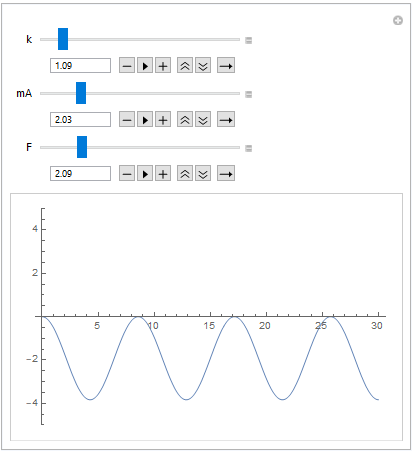
\includegraphics[width=0.7\linewidth]{screenshot010}
			\caption{Utilizamos valores mais ou menos proporcionais para cada uma das constantes do problema.}
			\label{fig:screenshot010}
		\end{figure}

	\end{solution}

	\clearpage

	\question Considere uma massa $ m $ rodando no extremo de um fio de comprimento $ R $. O movimento se dá em um plano vertical no campo gravitacional da Terra. Num determinado instante a velocidade da massa é $\vec{v}$ e o ângulo que o fio faz com a horizontal é $ \theta $, segundo a Fig. \ref{fig:fig5}.

	\begin{enumerate}[label=\alph*.]
		\item Desenhe o diagrama de forças atuando sobre a massa $ m $.
		\item Decomponha as forças nas direções $\rhat $ e $\that $.
		\item Encontre a força que o fio exerce sobre a massa $ m $.
		\item Qual a condição para que a massa $ m $ desenvolva uma trajetória circular e não caia dentro do círculo?
		\item  Encontre a aceleração tangencial nesse instante. Quando a velocidade da massa aumenta (diminui)?
	\end{enumerate}

	\begin{solution}

		\changelabel{(\alph*)}

		\begin{unindent}[start = 1]
			\item
		\end{unindent}

		\begin{multi}
			Sendo a situação como ilustrada na figura ao lado, já que está num plano vertical, podemos inferir que há a aceleração da gravidade atuando sobre o bloco e, portanto, temos a força peso $ \vec{P} $. Além disso, também há a força centrípeta, que ``puxa'' o bloco para a trajetória circular, e é aplicada pelo fio, portanto, trata-se de sua tensão $ \vec{T} $.

			\nextcol

			\centering
			\begin{tikzpicture}[scale=1.5]
				\draw[->] (-0.5,0) -- (2.5,0) node[right] {$ x $};
				\draw[->] (0,-0.5) -- (0,2.5) node[above] {$ y $};

				\draw[dotted] (-5:2cm) arc (-5:95:2cm);

				\coordinate (x) at (2.5,0);
				\coordinate (A) at (30:1.8);
				\coordinate (O) at (0,0);

				\pic[draw=black, angle radius=20pt,angle eccentricity=1,"$ \theta $" {xshift=5pt,yshift=1pt}] {angle=x--O--A};

				\draw[dashed] (0,0) -- (A);
				\draw (A) node[draw,fill=white,name=m,rectangle,minimum width=0.8cm,minimum height=0.5cm,anchor=south,rotate=-60] {$ m $};

				%			\draw[decorate,decoration={brace,raise=5pt,amplitude=8pt}] (0,0) -- node[rotate=30,yshift=20pt] {$ R $} (A);
				\draw[dashed] (0,0) -- +(-60:-0.5) (A) ++(-60:-0.25) -- +(-60:-0.25);
				\draw[thick] (-60:-0.4) -- (-60:-0.6) (A) ++(-60:-0.4) -- +(-60:-0.2);
				\draw[Stealth-Stealth] (-60:-0.5) -- node[rotate=30,above] {$ R $} +(A);

				\draw[-Latex] (m.west) -- node[above right] {$ \vec{v} $} +(-60:-0.8);
				\fill (0,0) circle (1.5pt) node[below left] {$ O $};

			\end{tikzpicture}
		\end{multi}

		\begin{center}
			\begin{tikzpicture}[x=3cm,y=3cm]
				\draw[->] (-0.5,0) -- (2.5,0) node[right] {$ x $};
				\draw[->] (0,-0.5) -- (0,2.5) node[above] {$ y $};

				\draw[dotted] (-5:2) arc (-5:95:2);

				\coordinate (x) at (2.5,0);
				\coordinate (A) at (30:2);
				\coordinate (O) at (0,0);

				\pic[draw=black, angle radius=40pt,angle eccentricity=1,"\LARGE $ \theta $" {xshift=13pt,yshift=3pt}] {angle=x--O--A};

				\draw[dashed] (0,0) -- (A);
				\filldraw (A) circle (5pt) node[right=5pt] {$ m $};

				%			\draw[decorate,decoration={brace,raise=5pt,amplitude=8pt}] (0,0) -- node[rotate=30,yshift=20pt] {$ R $} (A);
				\draw[dashed] (0,0) -- +(-60:-0.4) (A) -- +(-60:-0.4);
				\draw[thick] (-60:-0.3) -- +(-60:-0.2) (A) ++(-60:-0.3) -- +(-60:-0.2);
				\draw[Stealth-Stealth] (-60:-0.4) -- node[rotate=30,above] {$ R $} +(A);

				\draw[-Latex] (A) -- node[right] {$ \vec{P} $} +(0,-0.8);
				\draw[-Latex] (A) -- node[rotate=30,above] {$ \vec{T} $} +(30:-0.5);
				\fill (0,0) circle (3pt) node[below left] {$ O $};

			\end{tikzpicture}
		\end{center}

		\begin{unindent}
			\item Sendo $ T=|\vec{T}| $ e $ P=|\vec{P}| $, decompondo as forças, temos:
			\begin{gather*}
				\vec{T}=-T\,\rhat\\
				\vec{P}=-P\sin\theta\,\rhat -P\cos\theta\,\that
			\end{gather*}

			\item A força resultante do fio sobre a massa deve ser a tensão $ \vec{T} $.

			\item  Sabendo que
			\begin{gather}
				\dot{\rhat}=\dot{\theta}\cdot\that\label{eq:drhat}\\
				\dot{\that}=-\dot{\theta}\cdot\rhat\label{eq:dthat}
			\end{gather}
			tomemos $ \ddot{\vec{r}} $:
			\begin{align}
				\ddot{\vec{r}} & =\del{\dot{\vec{r}}}'=\del{\dot{r}\cdot\rhat+r\cdot\dot{\rhat}}'\nonumber                                                                                                 \\
				\intertext{substituindo \ref{eq:drhat}}
				               & =\del{\dot{r}\cdot\rhat+r\cdot\dot{\theta}\cdot\that}'\nonumber                                                                                                           \\
				               & =\ddot{r}\cdot\rhat+\dot{r}\cdot\dot{\rhat}+\dot{r}\cdot\dot{\theta}\cdot\that+r\del{\ddot{\theta}\cdot\that+\dot{\theta}\cdot\dot{\that}}\nonumber                       \\
				\intertext{substituindo \ref{eq:drhat} e \ref{eq:dthat}}
				               & =\ddot{r}\cdot\rhat+\dot{r}\cdot\dot{\theta}\cdot\that+\dot{r}\cdot\dot{\theta}\cdot\that+r\del{\ddot{\theta}\cdot\that-\dot{\theta}\cdot\dot{\theta}\cdot\rhat}\nonumber \\
				\ddot{\vec{r}} & =\del{\ddot{r}-r\cdot\dot{\theta}\cdot\dot{\theta}}\rhat+\del{2\dot{r}\cdot\dot{\theta}+r\cdot\ddot{\theta}}\that\label{eq:ddotr}
			\end{align}

			Sendo, então, a aceleração radial $ \vec{a_r} $ paralela à trajetória da massa, e a aceleração tangencial $ \vec{a_t} $ perpendicular à trajetória, temos
			\begin{gather}
				\vec{F_{r\parallel}}=m\,\vec{a_r}\label{eq:fpara}\\
				\vec{F_{r\perp}}=m\,\vec{a_t}\label{eq:fperp}
			\end{gather}

			Chamando $ \dot{\theta}=\omega $ e sabendo que a direção radial é simbolizada pelo vetor $ \rhat $, tomando o módulo de \ref{eq:fpara}, temos que:
			\begin{equation}\label{eq:fparacomp}
				\envert{\vec{F_{r\parallel}}}=|m\,\vec{a_r}|\implies -\del{T+P\sin\theta}=m\del{\ddot{r}-r\cdot\omega^{2}}
			\end{equation}

			Considerando $ P=m\,g $ (pela Segunda Lei de Newton), e sabendo que, para que o movimento seja circular, devemos ter $ r=R\implies \dot{r}=\dot{R}=0 $ (e, consequentemente, $ \ddot{R}=0 $), por \ref{eq:fparacomp}, temos
			\[ -\del{T+m\,g\sin\theta}=-m\,R\,\omega^{2}\implies
				T=m\del{R\,\omega^{2}-g\sin\theta} \]
			como o fio não pode empurrar a massa, $ T\stackrel{!}{\geqslant}0 $. Se usarmos a condição para o ponto onde $ T $ é mínimo (no topo da trajetória, quando temos $ \theta=\ang{90} $), temos a condição
			\begin{equation}\label{eq:tCond}
				T=m\del{R\,\omega^{2}-g}\geqslant0 \implies R\,\omega^{2}\geqslant g
			\end{equation}
			para que o movimento seja circular.

			\item Sabendo que a direção tangencial é simbolizada pelo vetor $ \that $, tomando o módulo de
			%		 $ \vec{a_t} $ de \ref{eq:ddotr} e 
			$\vec{a_t}=\vec{F_{r\perp}}/m$ (de \ref{eq:fperp}) e $ P=m\,g $, temos que
			\[ |\vec{a_t}|=\envert{\dfrac{\vec{F_{r\perp}}}{m}}=-\dfrac{P\cos\theta}{m}=-g\cos\theta, \]
			portanto, a velocidade do bloco aumenta na descida da massa (quando $ \cos\theta<0 $), e diminui na subida (quando $ \cos\theta>0 $).
		\end{unindent}
	\end{solution}



	\question Um bloco de massa $ m $ está em repouso sobre um plano inclinado de ângulo $ \theta $. O coeficiente de atrito é $ \mu $.

	\begin{enumerate}[label=\alph*.]
		\item Desenhe o diagrama de forças atuando sobre a massa $ m $.
		\item Escreva as equações de movimento para $ m $. Decomponha as forças convenientemente.
		\item Encontre o valor de $\theta$ para o qual o bloco começa a deslizar.
	\end{enumerate}

	\begin{solution}

		\changelabel{(\alph*)}

		\topenum
		\begin{multi}

			\centering
			\begin{tikzpicture}[xscale=-1,scale=3]

				\filldraw[fill=black!30!white] (0,0)
				-- +(30:2) -- (30:2|-0,0) coordinate (V) -- cycle;

				\draw (V) rectangle ++(-0.1,0.1) +(0.05,-0.05) circle (0.1pt);

				\begin{scope}[shift={(30:1)},rotate=30,x=0.1cm,y=0.1cm,scale=0.5]

					\coordinate (C) at (0,3);
					\node[right=-1pt,rotate=-30] at (C) {$ m $};
					\draw (-3,0) -- (3,0) -- ++(0,6) -- ++(-6,0) -- cycle;

					\draw[-Latex] (C) -- +(0,8) node[left=0pt,rotate=-30] {\footnotesize $ \vec{N} $};
					%			\draw[-Latex,blue!60!white] (C) -- node[above left,shift={(5pt,12pt)},rotate=60] {\footnotesize $ P\cdot\cos{\theta}  $} +(0,-10) coordinate (B);

					%			\draw[-Latex,blue!60!white] (C)++(0,-0.5) -- node[below right,rotate=-30,shift={(-5pt,2pt)}] {\tiny $ P\cdot\sin{\alpha} $} +(-5,0);
					\draw[-Latex] (C) -- +(7,0) node[above=0pt,rotate=-30] {\footnotesize $ \vec{F_{at}} $};

				\end{scope}

				\coordinate (A) at (30:2);
				\coordinate (O) at (0,0);
				\coordinate (B) at (2,0);

				\draw[-Latex] (C) -- +(0,-0.5) coordinate(P) node[right=0pt] {\footnotesize $ \vec{P} $};

				\path[name path=O--A] (O) -- (A);
				\path[name path=C--P] (C) -- (P);

				\path[name intersections={of=O--A and C--P,by=E}];

				\pic[draw,angle radius=10pt,angle eccentricity=1,"$ \mathsmaller{\theta} $" {xshift=1pt,yshift=-3pt}] {angle=P--E--O};

				\pic[draw,angle radius=20pt,angle eccentricity=1,"$ \theta $" {xshift=-5pt,yshift=1pt}] {angle=A--O--B};
			\end{tikzpicture}

			\nextcol

			Sejam $ \vec{P} $ o peso do bloco\footnote{Vamos adotar uma gravidade $ g $ que puxa o bloco para baixo.}, $ \vec{N} $ a normal da plano sobre o bloco e $ \vec{F_{at}} $ a força de atrito que segura o bloco para trás. A sua aceleração é $ \vec{a}=\vec{0} $, e pela segunda lei de Newton, temos:
			\begin{equation}\label{eq:motEqIP}
				\vec{P}+\vec{F_{at}}+\vec{N}=m\,\vec{a}=\vec{0}
			\end{equation}
		\end{multi}

		\begin{unindent}
			\item Como o movimento analisado é na superfície do bloco, vamos adotar um eixo de coordenadas com origem em seu centro, com a vertical na direção e sentido do vetor normal $ \vec{N} $ e a horizontal como paralela à superfície do plano e sentido positivo pra baixo.

			Adotemos a notação $ |\vec{v}|=v $.

			Dessa forma, podemos analisar a equação de movimento nas duas direções dos eixos definidos:
			\begin{gather}
				-P\sin\theta+N=0\implies N=P\sin\theta\label{eq:Nmod}\\
				P\cos\theta-F_{at}=m\,a\label{eq:PcosT}
			\end{gather}
			e queremos que $ a $ seja maior que zero, para que haja o deslizamento.\footnote{Repare que $ a\stackrel{!}{\geqslant}0 $ pois o atrito não pode puxar o bloco.} Sendo $ F_{at}=\mu\,N $, de \ref{eq:PcosT}, temos:
			\begin{align*}
				a          & =\dfrac{P\cos\theta-\mu\,N}{m}                                                    \\
				\intertext{substituindo \ref{eq:Nmod} e $ P=m\,g $, temos}
				a          & =g\del{\cos\theta-\mu\sin\theta}\stackrel{!}{>}0                                  \\
				\intertext{assumindo $ \cos\theta>0 $, temos}
				\tan\theta & \stackrel{!}{<}\dfrac{1}{\mu}                                                     \\
				\theta     & \stackrel{!}{<}\arctan\dfrac{1}{\mu}\qquad\text{para $ 0<\theta<\dfrac{\pi}{2} $}
			\end{align*}
		\end{unindent}

	\end{solution}

\end{questions}

\clearpage

\appendix

\begin{figure}[H]
	\fbox{
		\begin{minipage}{0.95\linewidth}
			\begin{multi}
				\smallskip
				\textbf{Mechanoelectrical transduction by hair cells.}

				\smallskip

				\textbf{A.} A tip link connects each stereocilium to the side of the longest adjacent stereocilium, as seen in a scanning electron micrograph (left) and a transmission electron micrograph (right) of a hair bundle’s top surface. Each tip link is only \SI{3}{\nano\meter} in diameter. The links appear stouter in the illustration on the left because of metallic coating during specimen preparation. (Reproduced, with permission, from Assad, Shepherd, and Corey 1991; reproduced, with permission, from Hudspeth and Gillespie 1994.)

				\smallskip

				\textbf{B. Top:} Ion flux through the channel that underlies mechanoelectrical transduction in hair cells is regulated by a molecular gate. The opening and closing of the gate are controlled by the tension in an elastic element, the gating spring, that senses hair-bundle displacement. (Adapted, with permission, from Howard and Hudspeth 1988.)

				\smallskip

				\textbf{Bottom:} When the hair bundle is at rest each transduction channel clatters between closed and open states, spending most of its time shut. Displacement of the bundle in the positive direction increases the tension in the gating spring, here assumed to be in part a tip link, attached to each channel’s molecular gate. The enhanced tension promotes channel opening and the influx of cations, thereby producing a depolarizing receptor potential. (Adapted, with permission, from Hudspeth 1989.)

				\nextcol

				A

				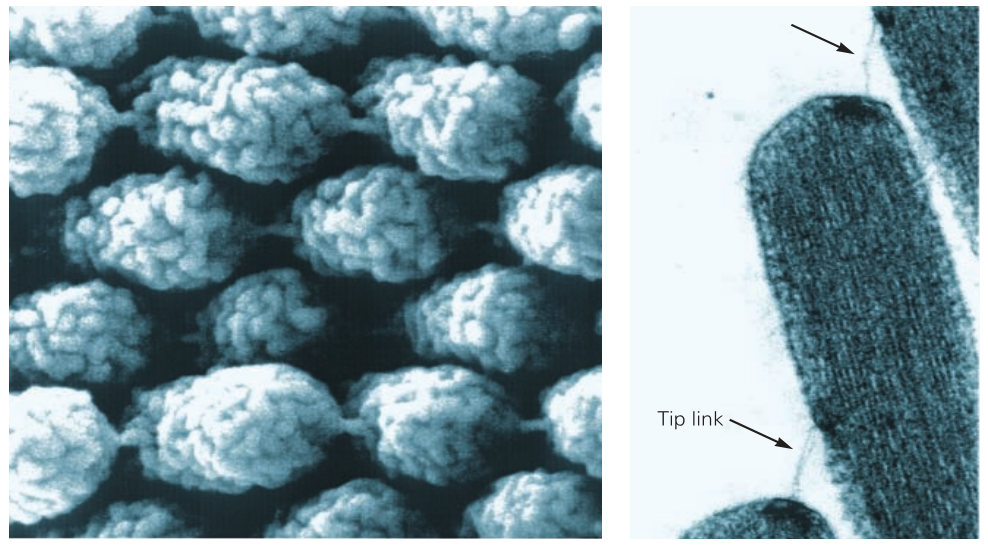
\includegraphics[width=1\linewidth]{screenshot009}

				B

				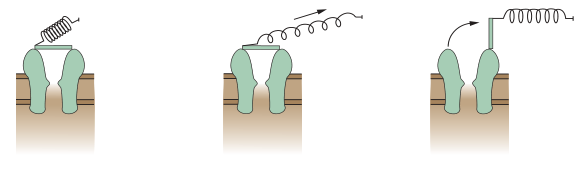
\includegraphics[width=1\linewidth]{screenshot005}

				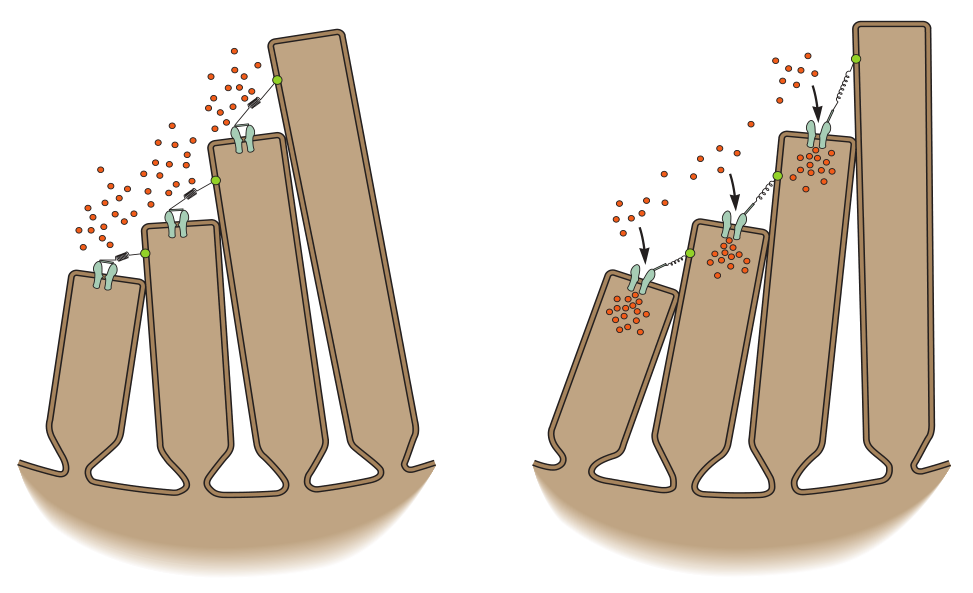
\includegraphics[width=1\linewidth]{screenshot006}
			\end{multi}

			\medskip

			\textbf{The Temporal Responsiveness of Hair Cells Determines Their Sensitivity}

			The mechanical sensitivity of hair cells is not constant; responsiveness varies in such a way that a given cell best detects behaviorally relevant stimuli. When it is to relatively low frequencies, the response to a stimulus of moderate intensity has a time constant of only \SI{80}{\micro\second} at room temperature. For mammals to be able to respond to frequencies greater than \SI{100}{\kilo\hertz}, the hair cells evidently display gating rates that are an order of magnitude greater.
		\end{minipage}
	}


	\caption{Modelo eletromecânico de transdução de movimento no ouvido.}
	\label{fig:fig3}
\end{figure}

\clearpage

\begin{figure}[H]
	\centering
	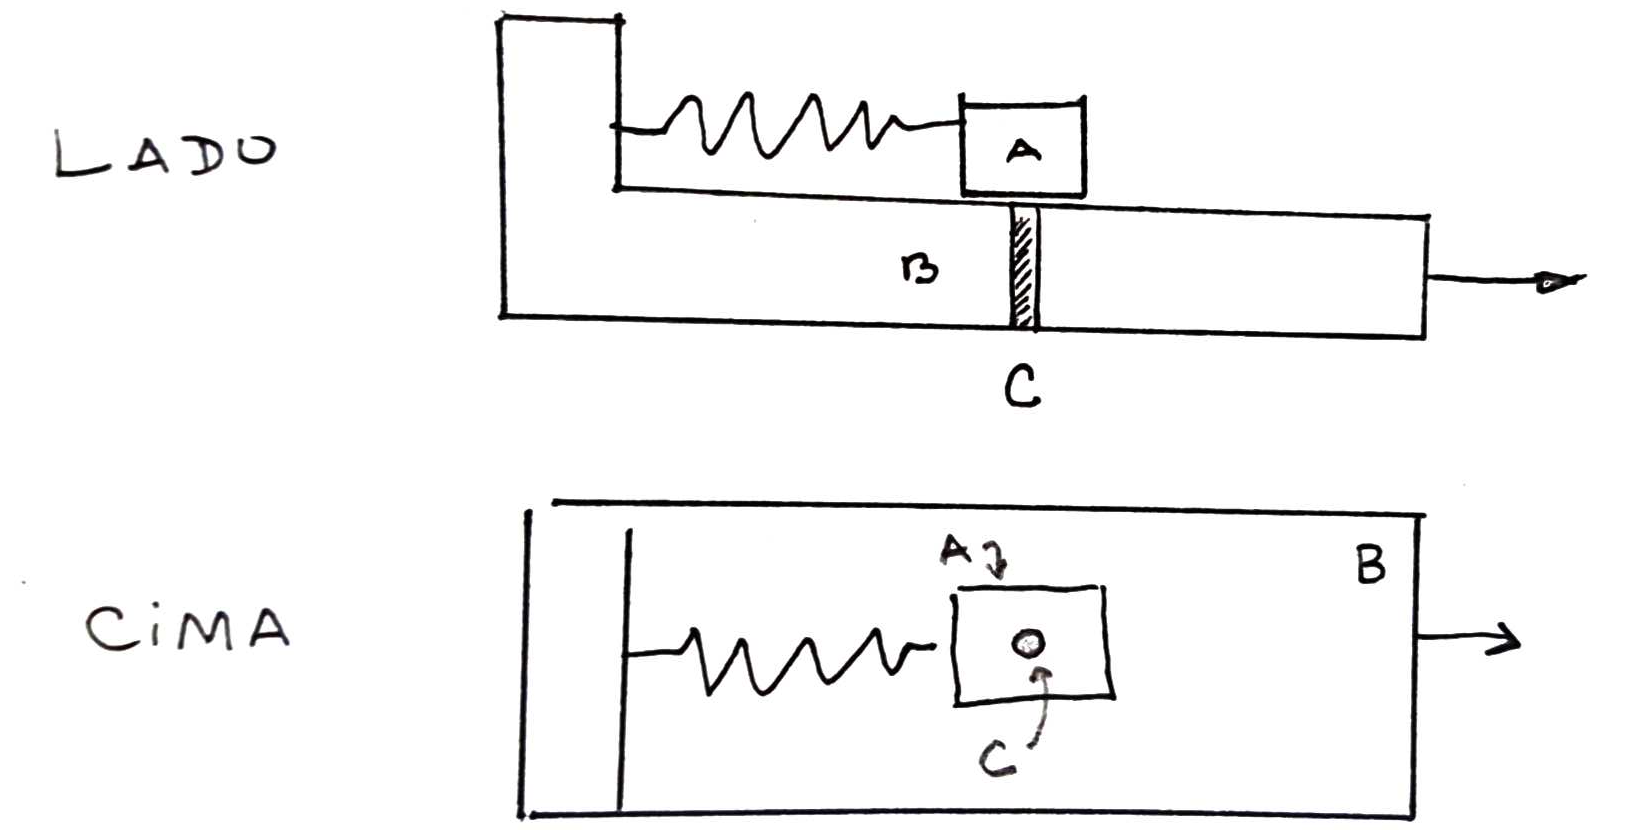
\includegraphics[width=0.5\linewidth]{screenshot007}
	\caption{Vista de cima e de lado. O canal $ C $ não entra, não tem nenhum efeito neste modelo. Não há atrito.}
	\label{fig:fig4}
\end{figure}

\bigskip

\begin{figure}[H]
	\centering
	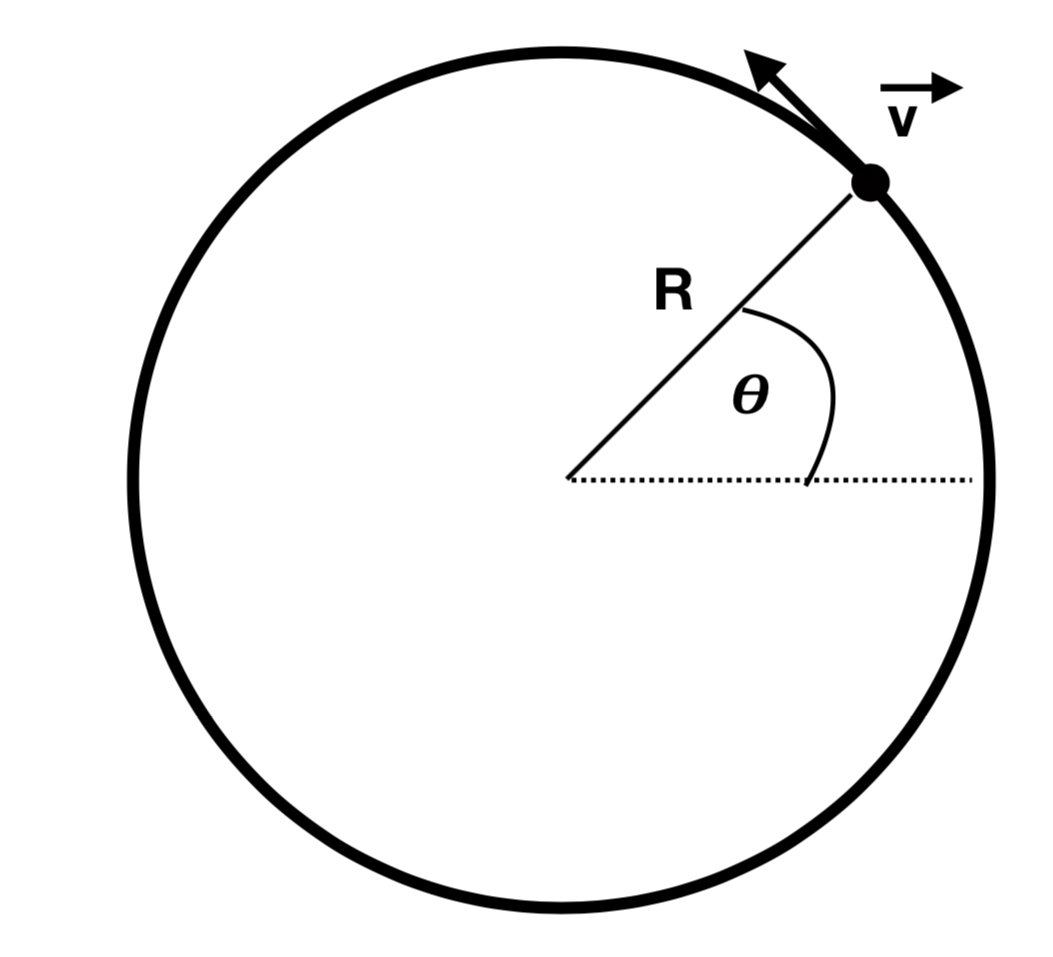
\includegraphics[width=0.4\linewidth]{screenshot008}
	\caption{Massa girando no campo gravitacional da Terra.}
	\label{fig:fig5}
\end{figure}

\end{document}